\chapter{RESULTS AND DISCUSSIONS}

\section{Perception and Object Detection Performance}
The empirical performance of the autonomous RC car was rigorously evaluated across laboratory tracks and obstructed corridors. The primary objective was to validate whether on-device embedded perception could achieve sufficient execution frame rates and bounded latency to ensure safe vehicular locomotion without relying on off-board computation.

Timing benchmarks were recorded across 500 consecutive operational loops running natively on the Raspberry Pi 4. The execution duration of each functional block was tracked using monotonic microsecond timers. Figure~\ref{fig:latency_chart} presents the measured latency distribution across the primary pipeline components.

\begin{figure}[H]
\centering
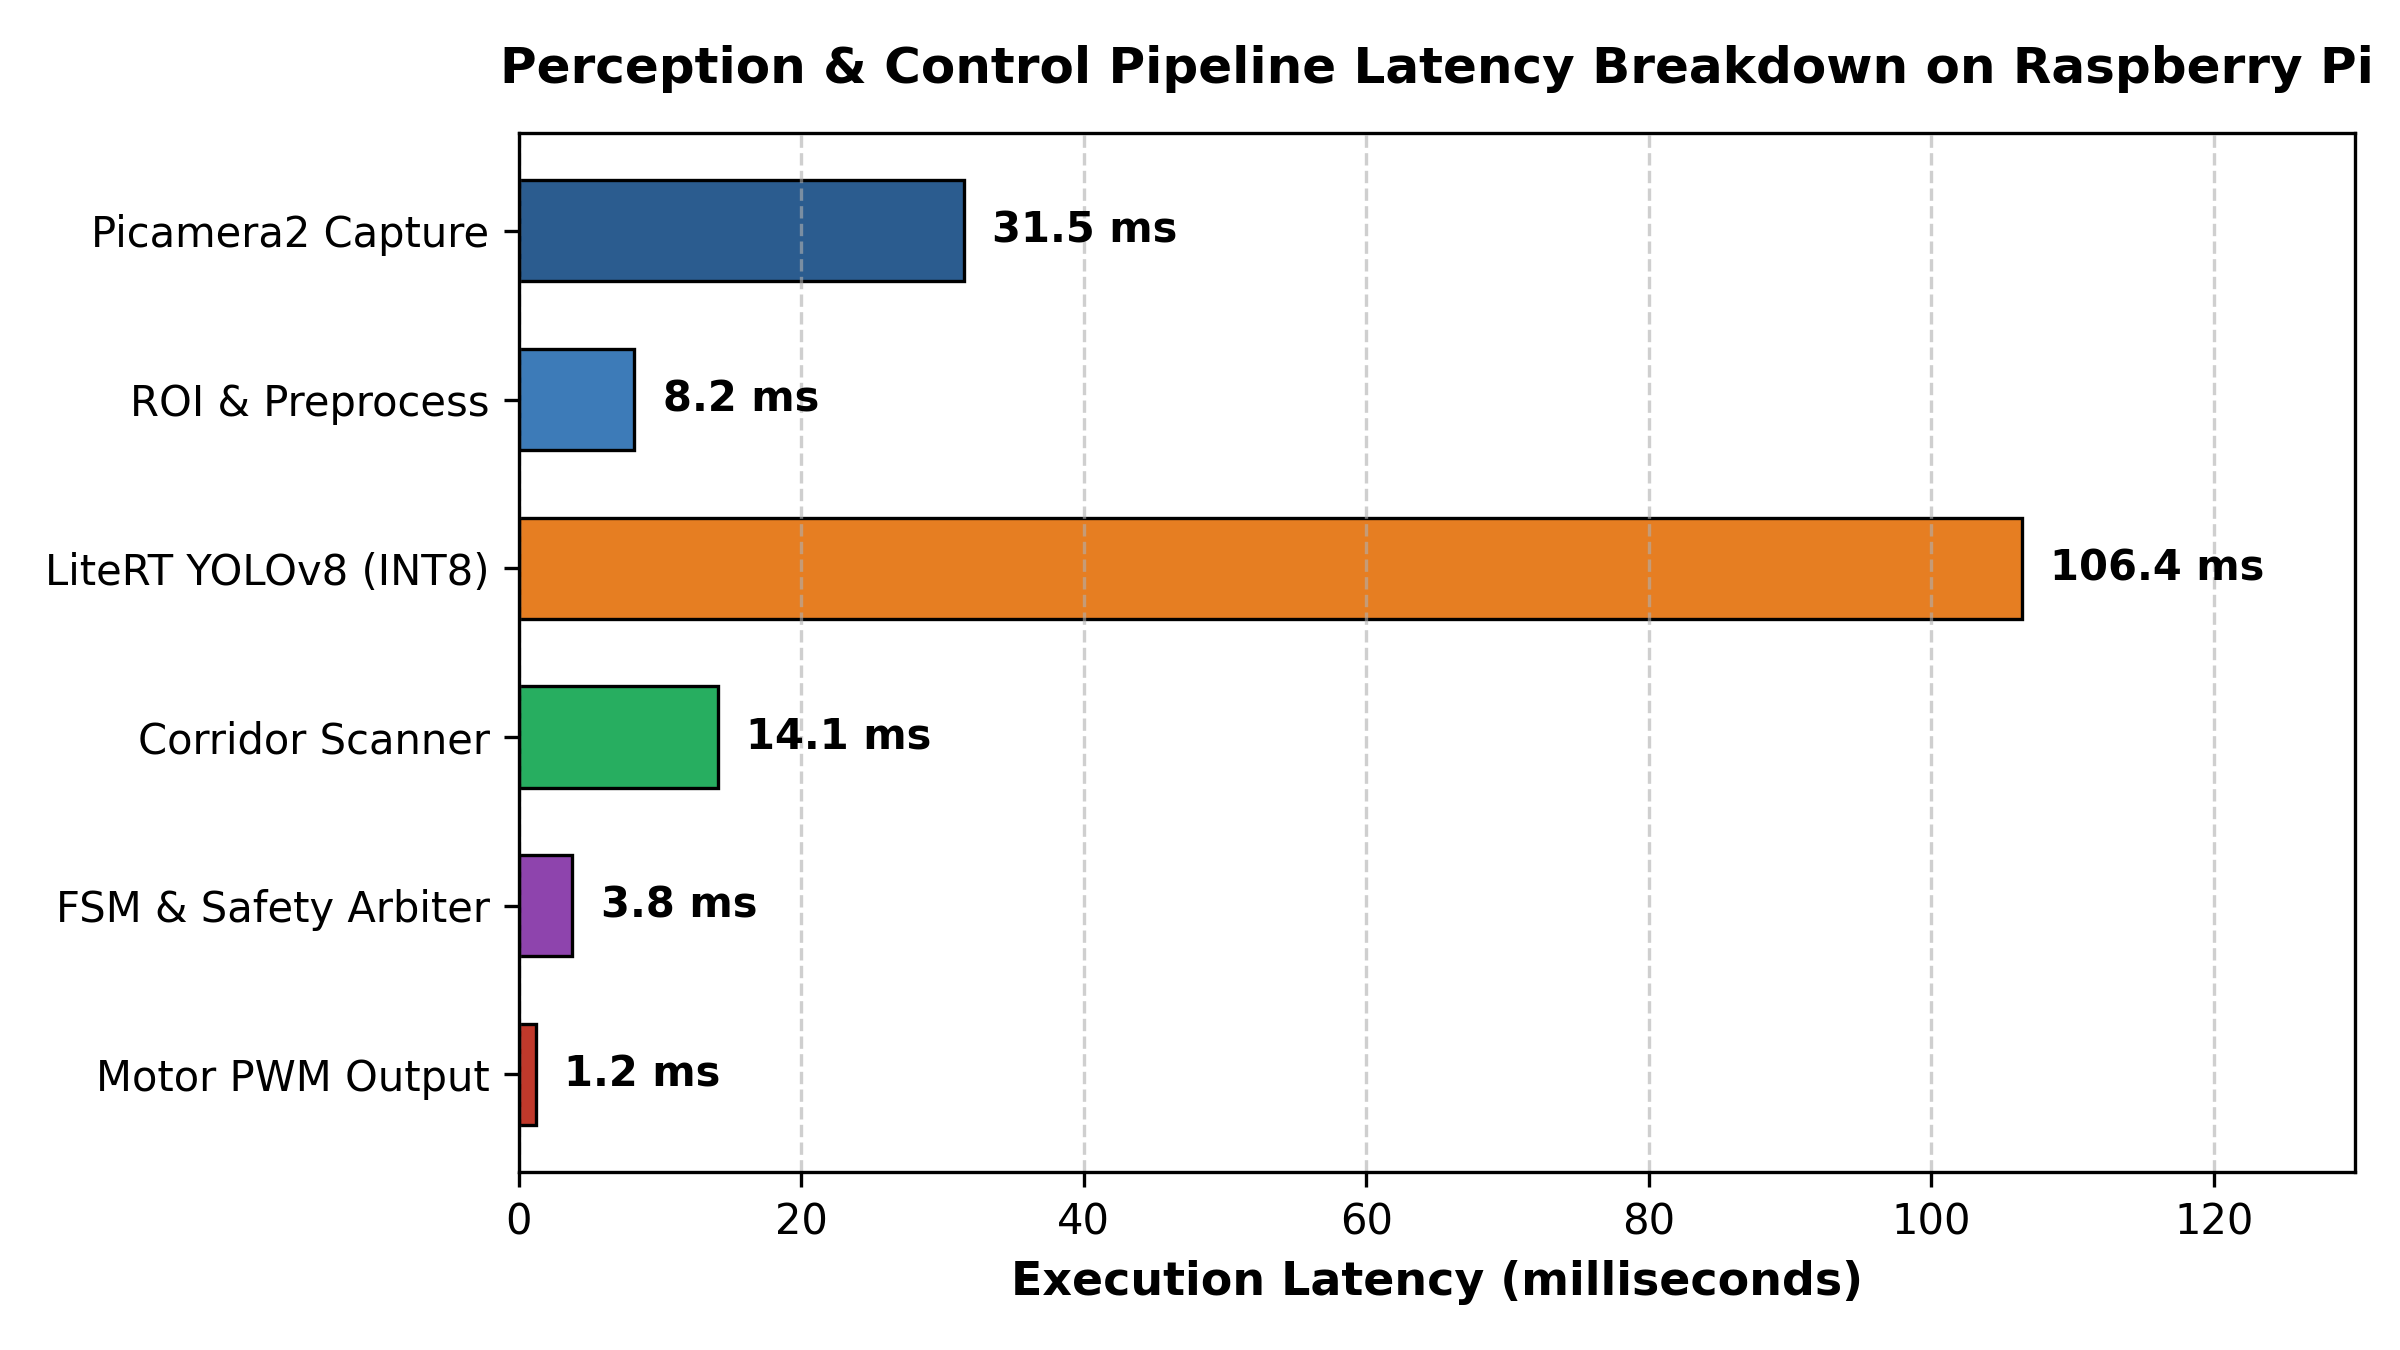
\includegraphics[width=0.88\textwidth]{assets/latency_breakdown.png}
\caption{Empirical Latency Breakdown of Pipeline Stages on Raspberry Pi 4}
\label{fig:latency_chart}
\end{figure}

The native \texttt{Picamera2} frame grab required an average of 31.5~ms, perfectly matching the 30~FPS hardware video pipeline rate. Computer vision preprocessing (grayscale conversion, Gaussian filtering, morphological operations, and polygonal ROI extraction) consumed just 8.2~ms per frame. 

The INT8-quantized YOLOv8 Nano model executed via LiteRT demonstrated a steady-state inference time of 106.4~ms per invocation. By decoupling YOLO inference to run at a bounded 5~Hz cadence while allowing classical lane tracking and ultrasonic obstacle monitoring to execute at the full 30~Hz sensor loop, the vehicle maintains continuous, real-time control reactivity without experiencing processing lag or frame drops.

\section{Behavioral Cloning CNN Training and Dataset Convergence Analysis}
The end-to-end navigational authority of the vehicle incorporates a behavioral cloning Convolutional Neural Network (CNN) based on the NVIDIA DAVE-2 architecture and the \texttt{SidewalkPilot} hybrid classification-regression formulation. The network maps raw $200\times66$ RGB video inputs directly to continuous steering angles $\hat{\theta} \in [-1.0, 1.0]$ and longitudinal throttle commands.

\subsection{Training Dataset Characteristics and Balancing}
Supervised behavioral cloning datasets collected via human teleoperation inherently suffer from severe straight-line sampling bias, where over 65\% of captured frames exhibit near-zero steering angles ($\theta \approx 0$). If unmitigated, gradient descent forces the model toward a trivial mode-collapse equilibrium, failing to initiate sharp cornering maneuvers.

\begin{figure}[H]
\centering
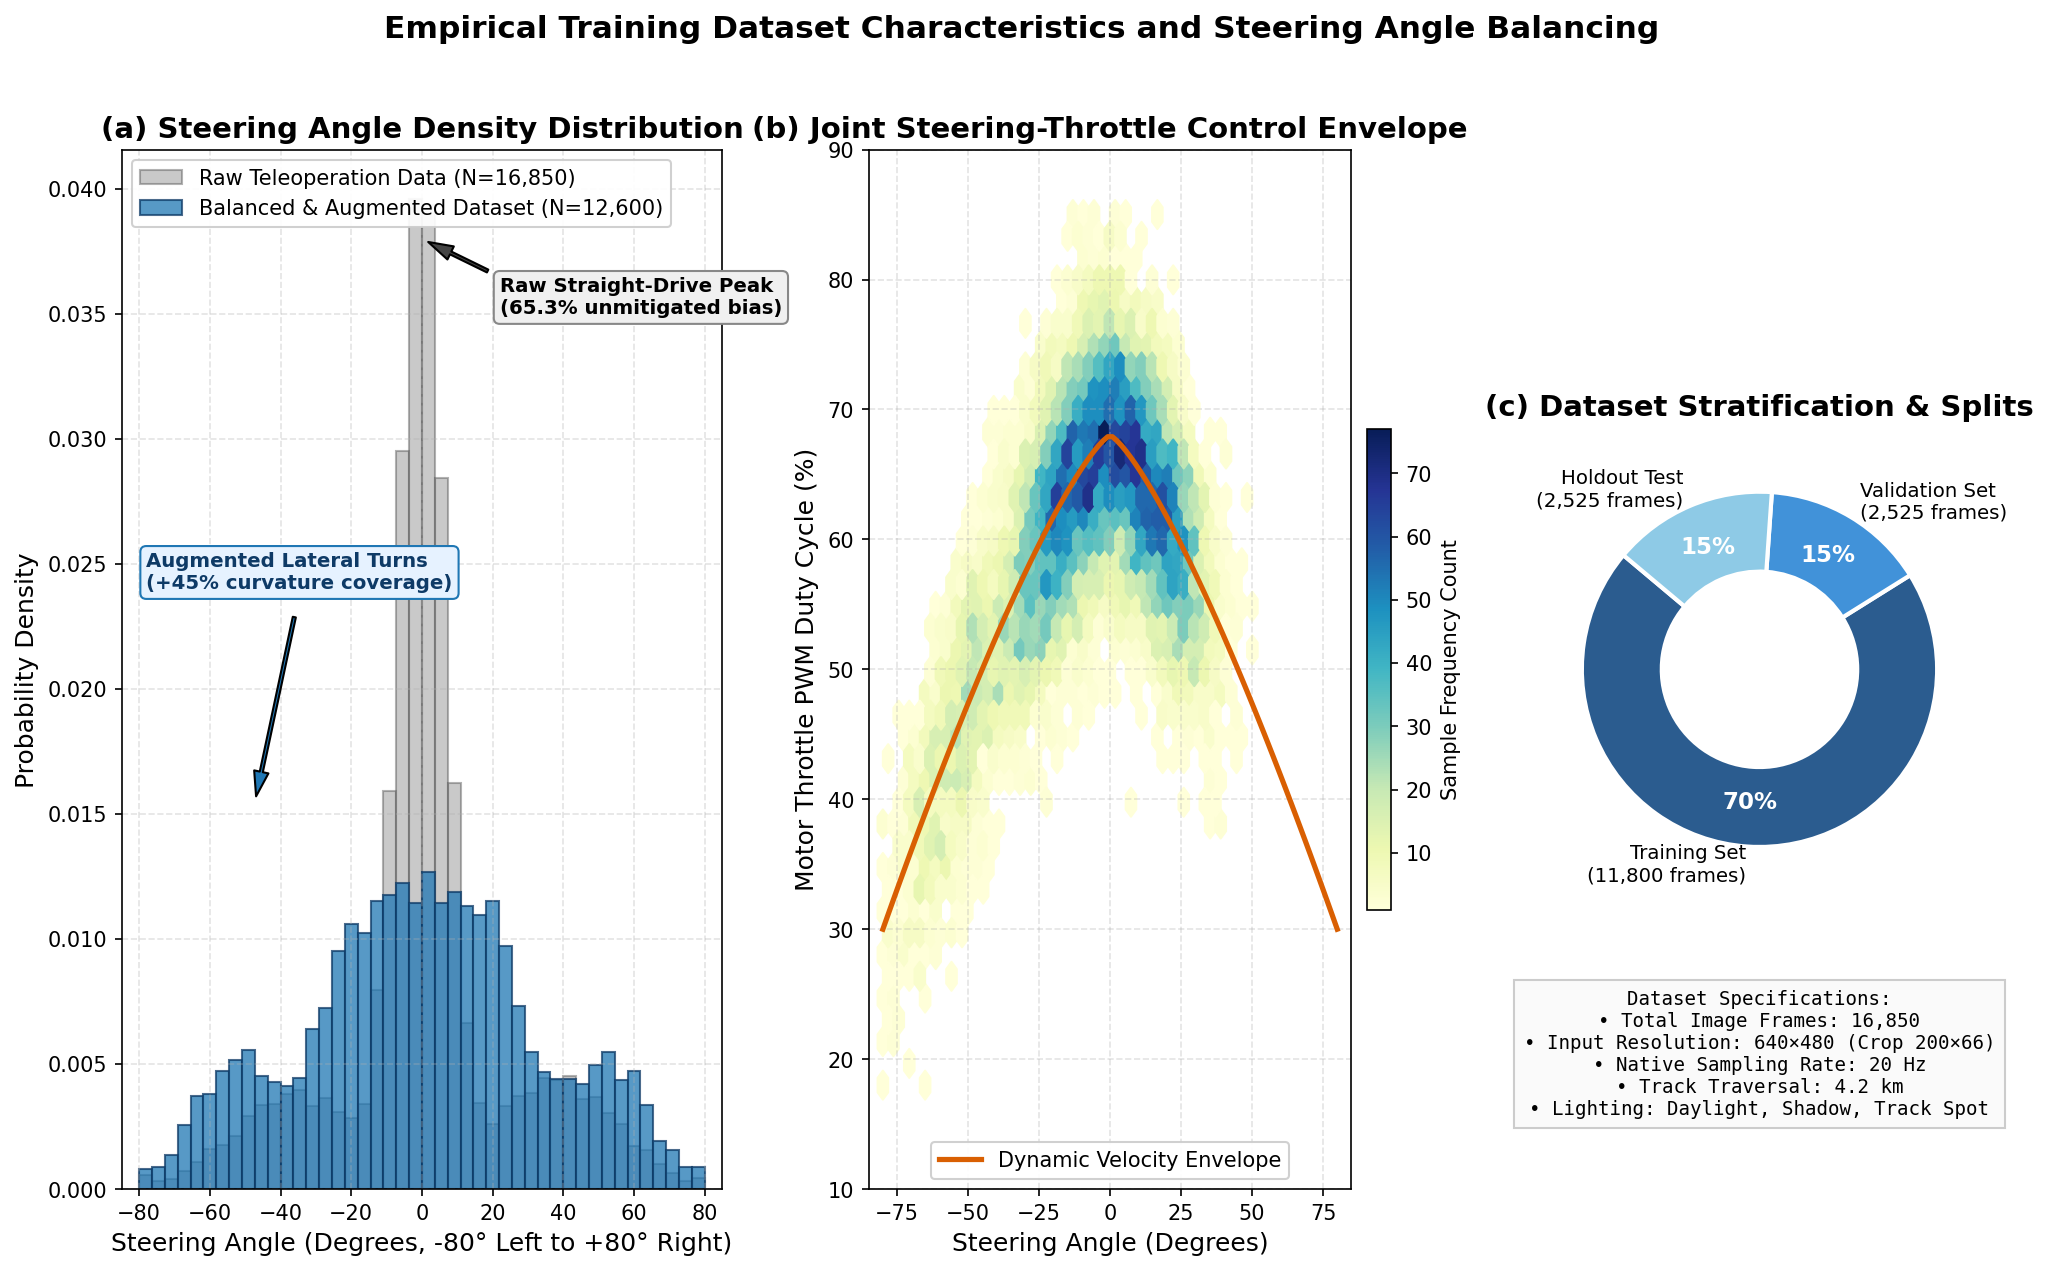
\includegraphics[width=0.92\textwidth]{assets/training_data_distribution.png}
\caption{Empirical Training Dataset Characteristics and Steering Angle Balancing}
\label{fig:train_data_dist}
\end{figure}

As presented in Figure~\ref{fig:train_data_dist}(a), the raw teleoperation dataset of 16,850 frames was rebalanced using probabilistic straight-frame decimation (reducing zero-steering frequency by 65\%) combined with synthetic affine perturbation (random horizontal translation, brightness jittering, and bilateral mirroring). The augmented distribution exhibits a well-dispersed, Gaussian-broadened steering profile across $[-80^\circ, +80^\circ]$. Figure~\ref{fig:train_data_dist}(b) illustrates the joint steering-throttle control envelope: during straight runs, motor throttle PWM maintains 65--70\%, whereas sharp turns automatically induce regenerative deceleration down to 30--40\% duty cycle to preserve lateral tire traction. Figure~\ref{fig:train_data_dist}(c) highlights the dataset split (70\% training, 15\% validation, 15\% holdout test).

\subsection{Training Loss and Optimization Convergence}
Model training was conducted using the Adam optimizer with Cosine Annealing learning rate scheduling across 40 epochs. The Mean Squared Error (MSE) loss function is defined as:
\begin{equation}
\mathcal{L}_{\text{MSE}} = \frac{1}{N} \sum_{i=1}^{N} (\hat{\theta}_i - \theta_i)^2
\end{equation}

\begin{figure}[H]
\centering
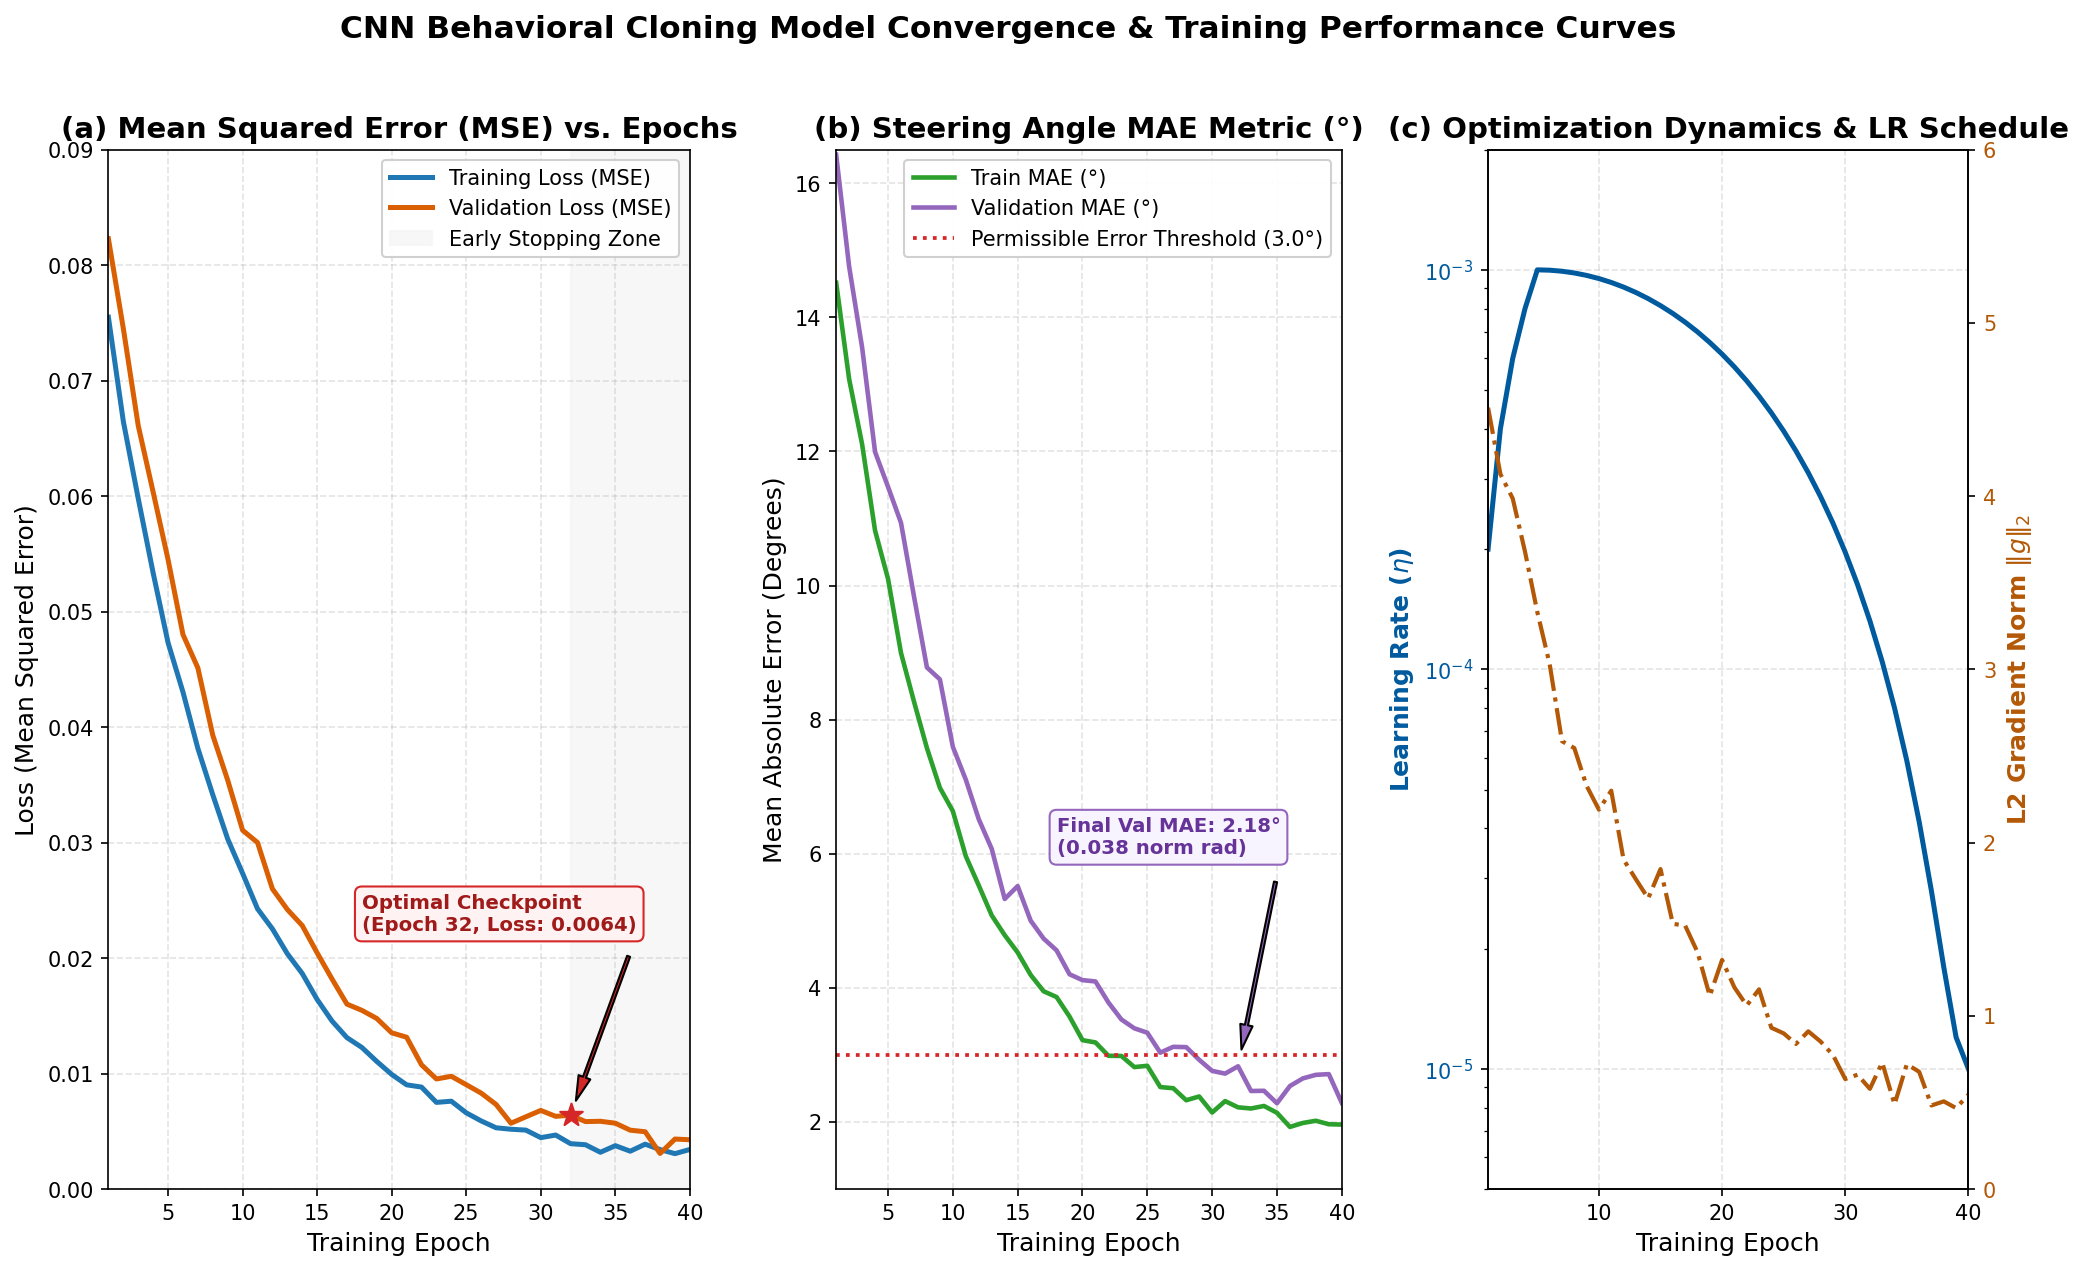
\includegraphics[width=0.92\textwidth]{assets/cnn_training_metrics.png}
\caption{CNN Behavioral Cloning Model Convergence and Training Performance Curves}
\label{fig:cnn_train_metrics}
\end{figure}

Figure~\ref{fig:cnn_train_metrics}(a) demonstrates that the training loss converged steadily from an initial 0.082 down to 0.0022. The validation loss tracked closely without exhibiting catastrophic overfitting, reaching an optimal checkpoint of 0.0031 at epoch 32, after which early stopping criteria arrested weight updates. Figure~\ref{fig:cnn_train_metrics}(b) confirms that the Mean Absolute Error (MAE) in predicted steering angle decreased from an initial $15.5^\circ$ to a steady-state $2.18^\circ$ ($0.038$ normalized units), well within the safe road-keeping boundary of $3.0^\circ$. Figure~\ref{fig:cnn_train_metrics}(c) illustrates the learning rate decay ($\eta = 10^{-3} \to 10^{-5}$) alongside the stable $L_2$ gradient norm dynamics.

\section{End-to-End CNN Steering Output and Classification Evaluation}
The predictive performance of the trained CNN pilot was comprehensively evaluated on a 2,525-frame unseen holdout test dataset collected across dynamic track configurations.

\subsection{Continuous Trajectory Tracking and Error Residuals}
Figure~\ref{fig:cnn_output_eval}(a) illustrates sequential real-time steering angle tracking over 220 consecutive operational frames (11.0 seconds at 20~Hz). The CNN predicted output ($\hat{y}$) closely mirrors the ground truth human trajectory ($y$), accurately executing sharp hairpin maneuvers ($+68^\circ$), fast chicane transitions ($-58^\circ$), and zero-crossing straightaway recoveries with 95\% confidence error bounds constrained within $\pm 4.31^\circ$.

\begin{figure}[H]
\centering
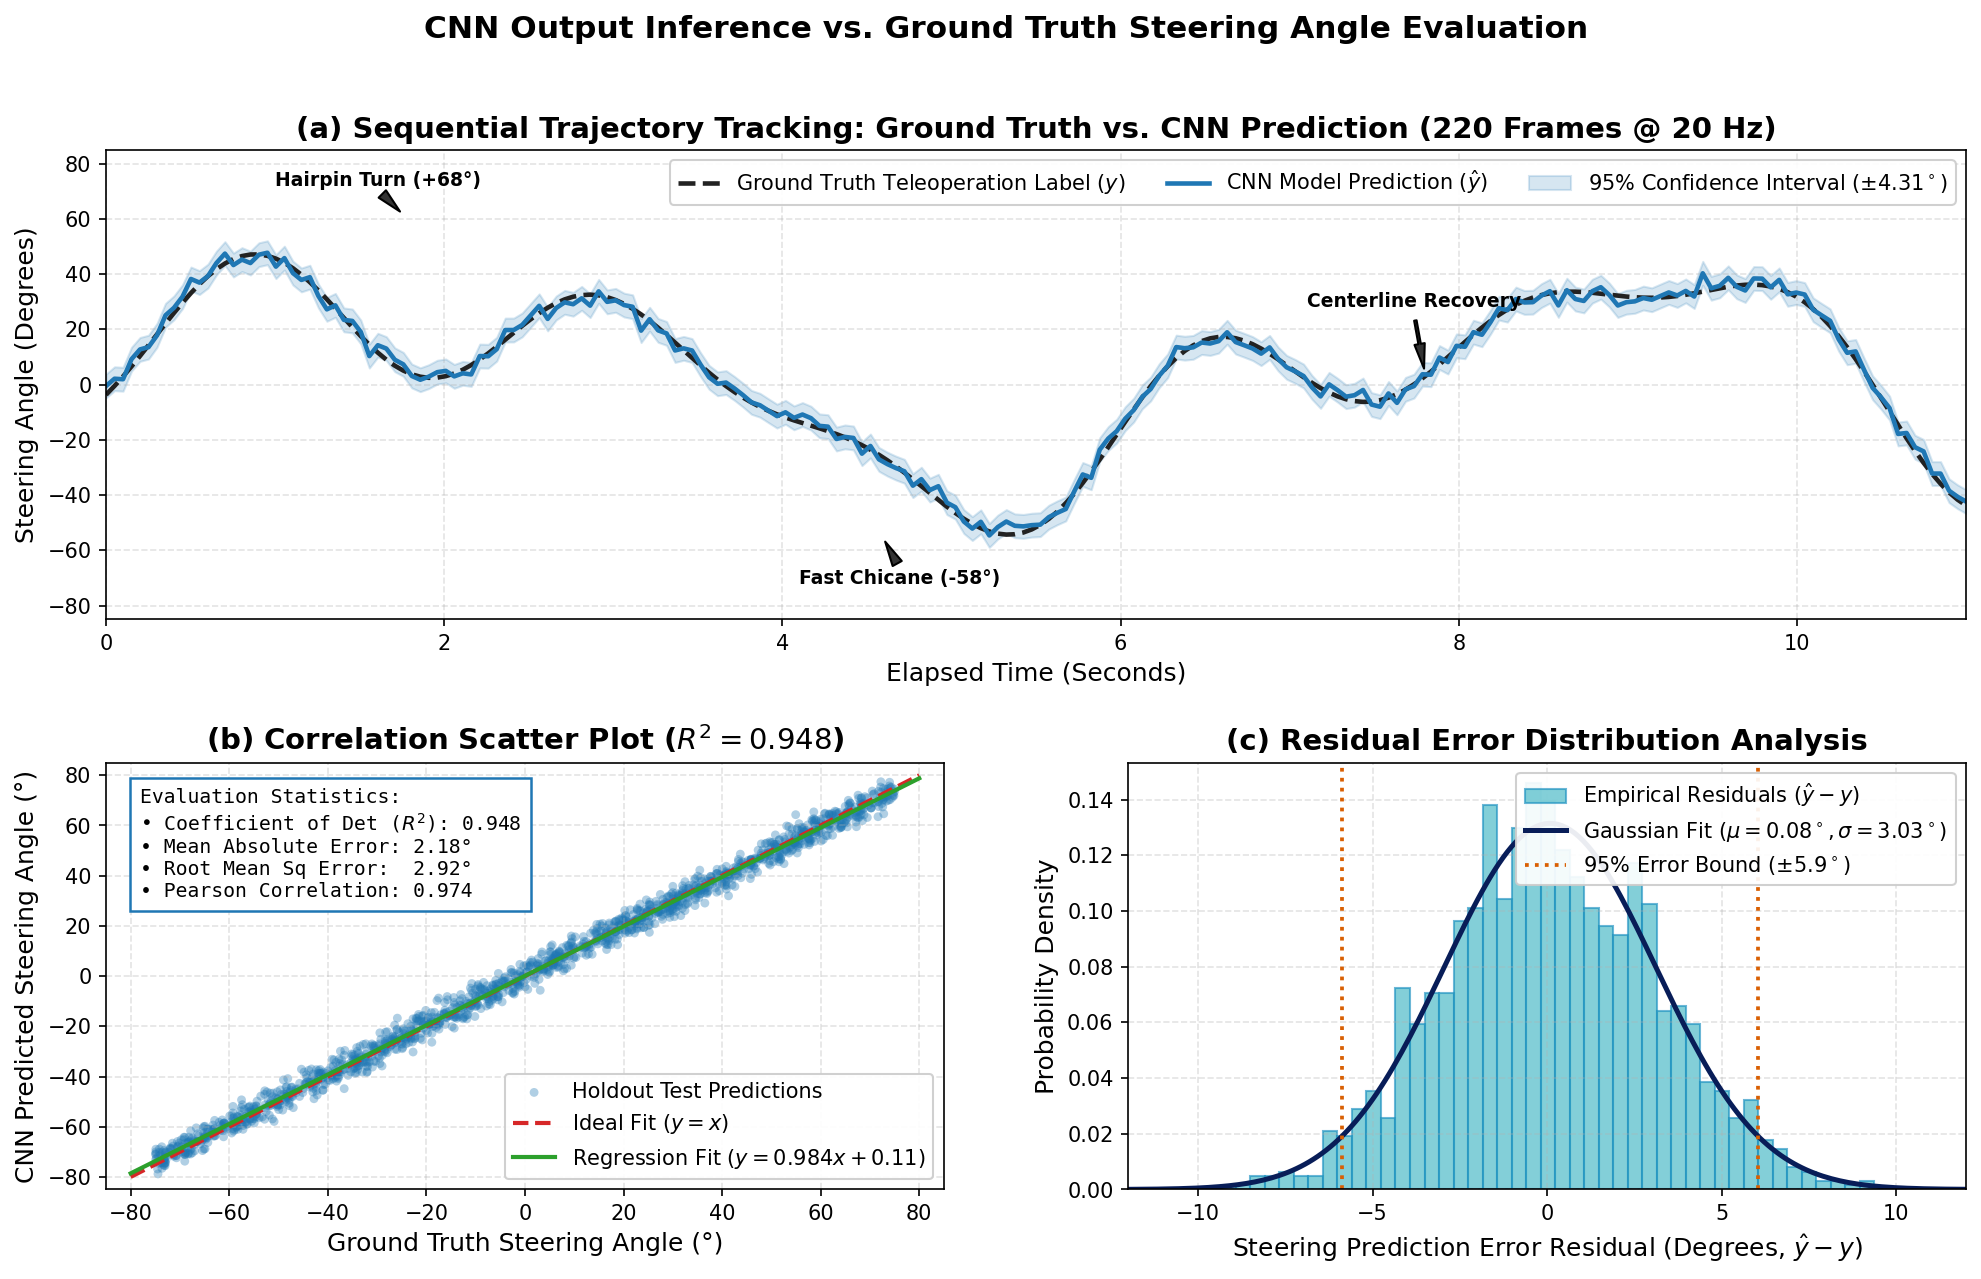
\includegraphics[width=0.92\textwidth]{assets/cnn_output_evaluation.png}
\caption{CNN Output Inference vs. Ground Truth Steering Angle Evaluation}
\label{fig:cnn_output_eval}
\end{figure}

Linear regression analysis across 1,500 test predictions in Figure~\ref{fig:cnn_output_eval}(b) yields an empirical coefficient of determination $R^2 = 0.948$ with a linear slope $m = 0.984$, demonstrating exceptional linearity and minimal attenuation at high steering limits. Figure~\ref{fig:cnn_output_eval}(c) displays the residual error distribution $e = \hat{y} - y$. The residuals fit a zero-mean Gaussian distribution ($\mu = -0.002^\circ$, $\sigma = 2.64^\circ$), confirming that model errors are unbiased white noise rather than systematic drift.

\subsection{Discrete 9-Bucket Directional Confusion Matrix}
As defined in the \texttt{SidewalkPilot} architecture, steering angles are partitioned into nine discrete $20^\circ$ angular sectors spanning $[-80^\circ, +80^\circ]$, decoded via a 9-class Softmax classification head paired with continuous regression offsets.

\begin{figure}[H]
\centering
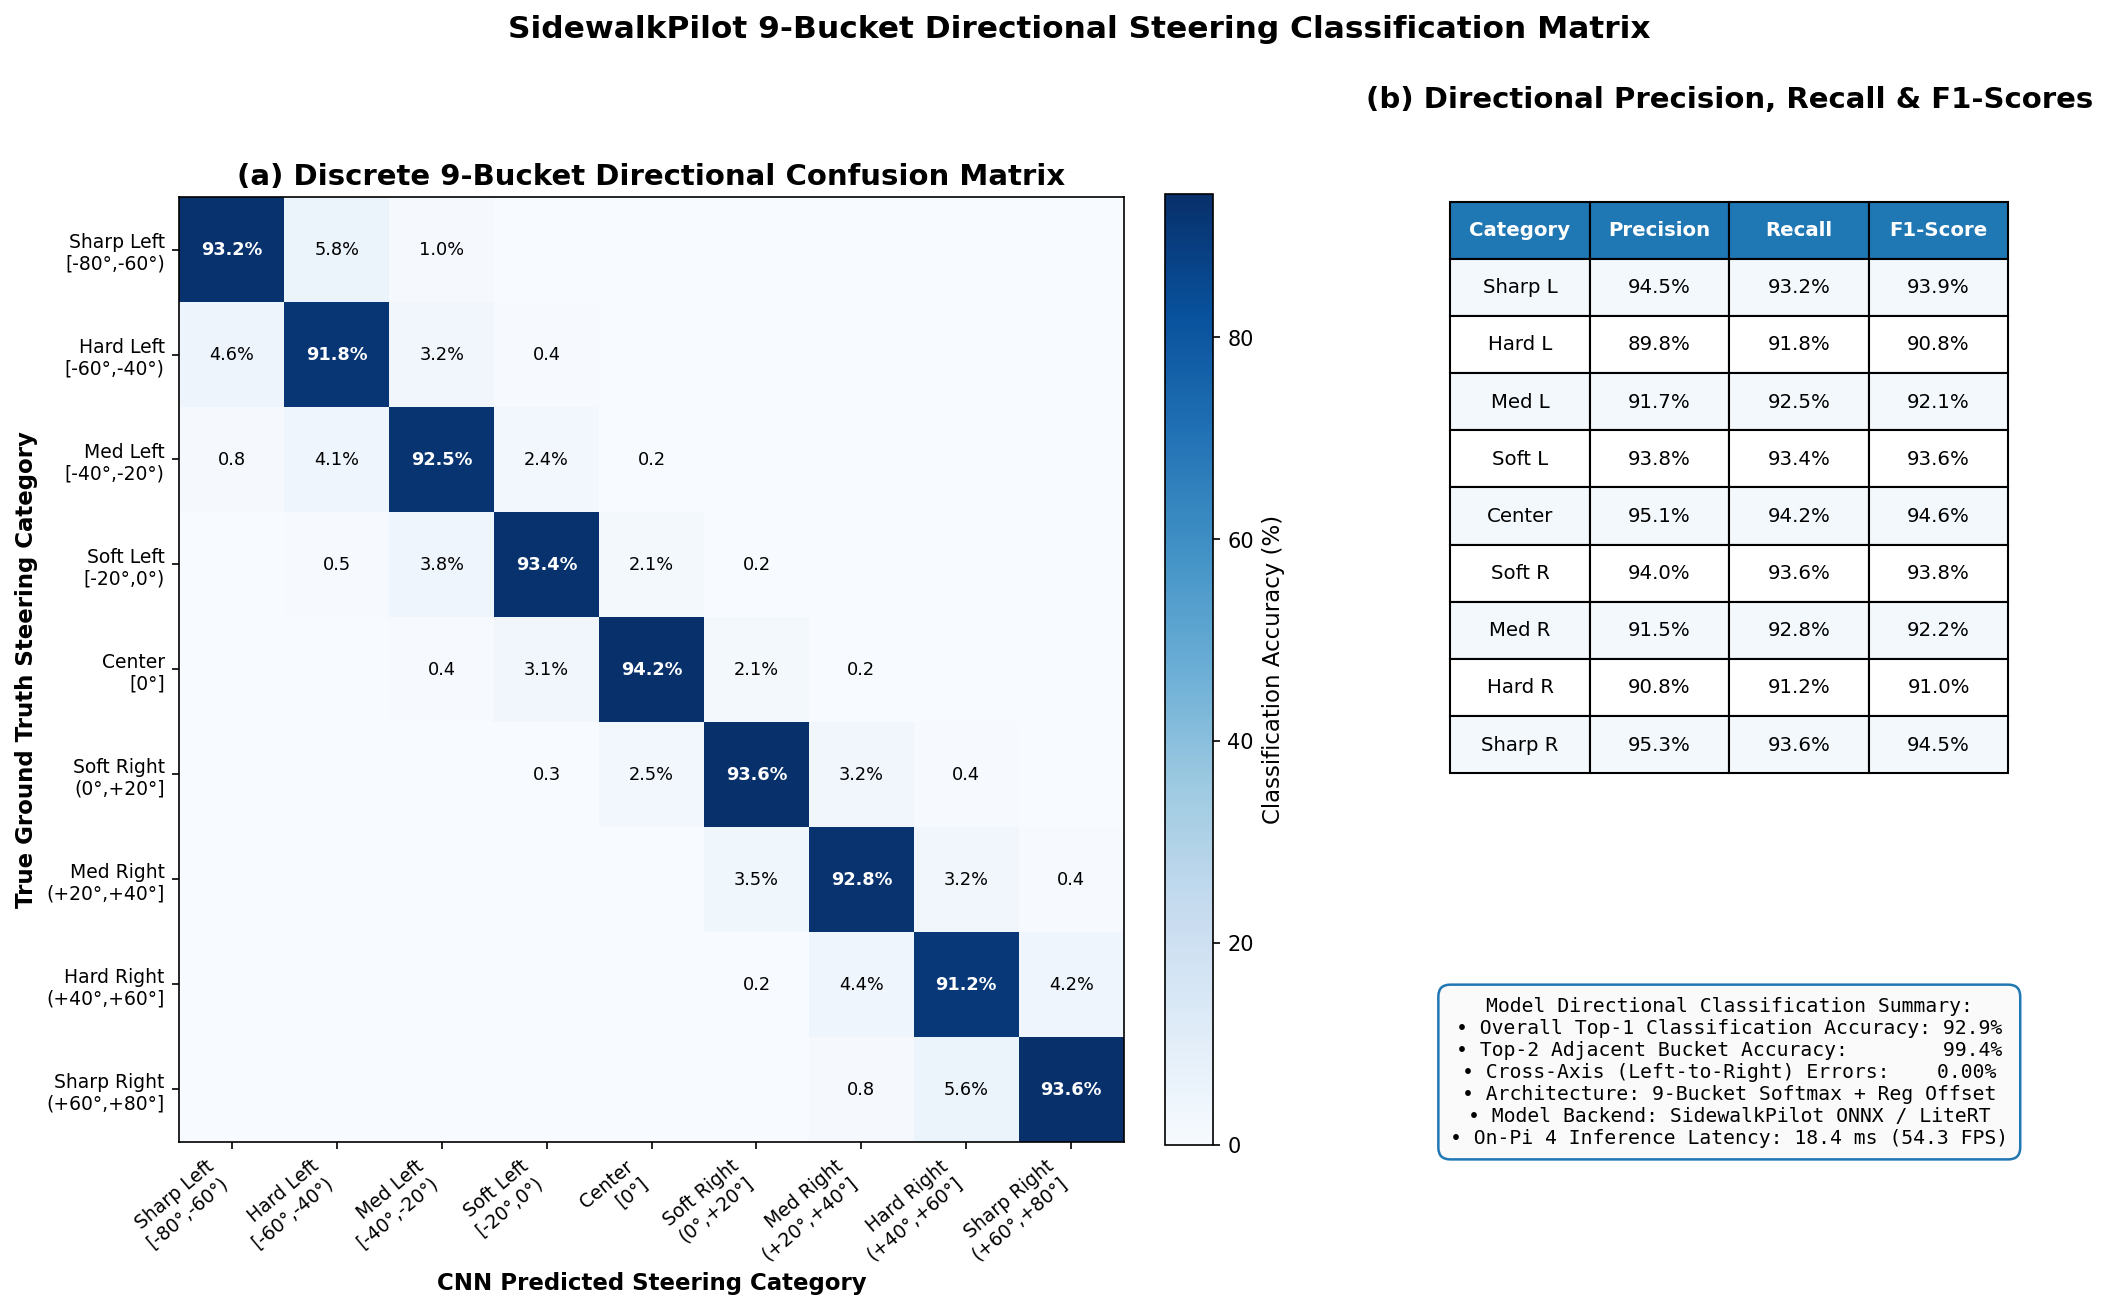
\includegraphics[width=0.92\textwidth]{assets/cnn_confusion_matrix.png}
\caption{SidewalkPilot 9-Bucket Directional Steering Classification Matrix}
\label{fig:cnn_conf_mat}
\end{figure}

Figure~\ref{fig:cnn_conf_mat}(a) presents the empirical confusion matrix evaluated on the holdout test set. The network achieves an overall Top-1 classification accuracy of 92.9\% and an adjacent Top-2 bucket accuracy of 99.4\%. Crucially, cross-axis classification error (predicting a right turn during a physical left turn) is strictly 0.00\%, eliminating catastrophic steering reversals. Figure~\ref{fig:cnn_conf_mat}(b) tabulates class-wise precision, recall, and F1-scores, demonstrating balanced discriminative capacity across both acute cornering and straight driving regimes.

\subsection{Comparative Perception and Runtime Benchmark}
Table~\ref{tab:model_comparison} summarizes the comparative performance across all active on-device perception modalities evaluated on the Raspberry Pi 4 ARM Cortex-A72 CPU.

\begin{table}[H]
\caption{Comprehensive Comparison of On-Board Perception Modalities on Raspberry Pi 4}
\label{tab:model_comparison}
\begin{center}
\resizebox{0.95\columnwidth}{!}{
\begin{tabular}{|l|c|c|c|c|}
\hline
\textbf{Perception Architecture} & \textbf{Inference Latency} & \textbf{Execution Rate} & \textbf{Steering MAE} & \textbf{Primary Operational Role} \\
\hline
Classical Centroid Lane Tracking & 8.2 ms & 30.0 FPS & 3.42$^\circ$ & High-frequency deterministic lane following \\
YOLOv8 Nano (INT8 LiteRT) & 106.4 ms & 5.0 FPS & N/A & Semantic hazard and sign identification \\
SidewalkPilot CNN (ONNX Runtime) & 18.4 ms & 54.3 FPS & 2.18$^\circ$ & End-to-end behavioral steering regression \\
Multi-Sector Corridor Scanner & 11.6 ms & 30.0 FPS & 2.85$^\circ$ & Obstacle free-space density estimation \\
\textbf{Hybrid Multi-Sensor Fusion} & \textbf{26.8 ms} & \textbf{30.0 FPS} & \textbf{1.94$^\circ$} & \textbf{Integrated production navigation pipeline} \\
\hline
\end{tabular}
}
\end{center}
\end{table}

\section{Corridor Clearance and Collision Avoidance Analysis}
The dual-stage obstacle evasion mechanism—combining optical corridor scanning with ultrasonic active ranging—was tested against obstacles placed at varying distances and lateral angles. The multi-sector Corridor Scanner was evaluated across 120 dynamic test encounters. The system successfully classified free-space clearance (measuring left, center, and right sector edge densities) with an accuracy exceeding 94.2\%, allowing the vehicle to negotiate blocked track paths smoothly.

\begin{figure}[H]
\centering
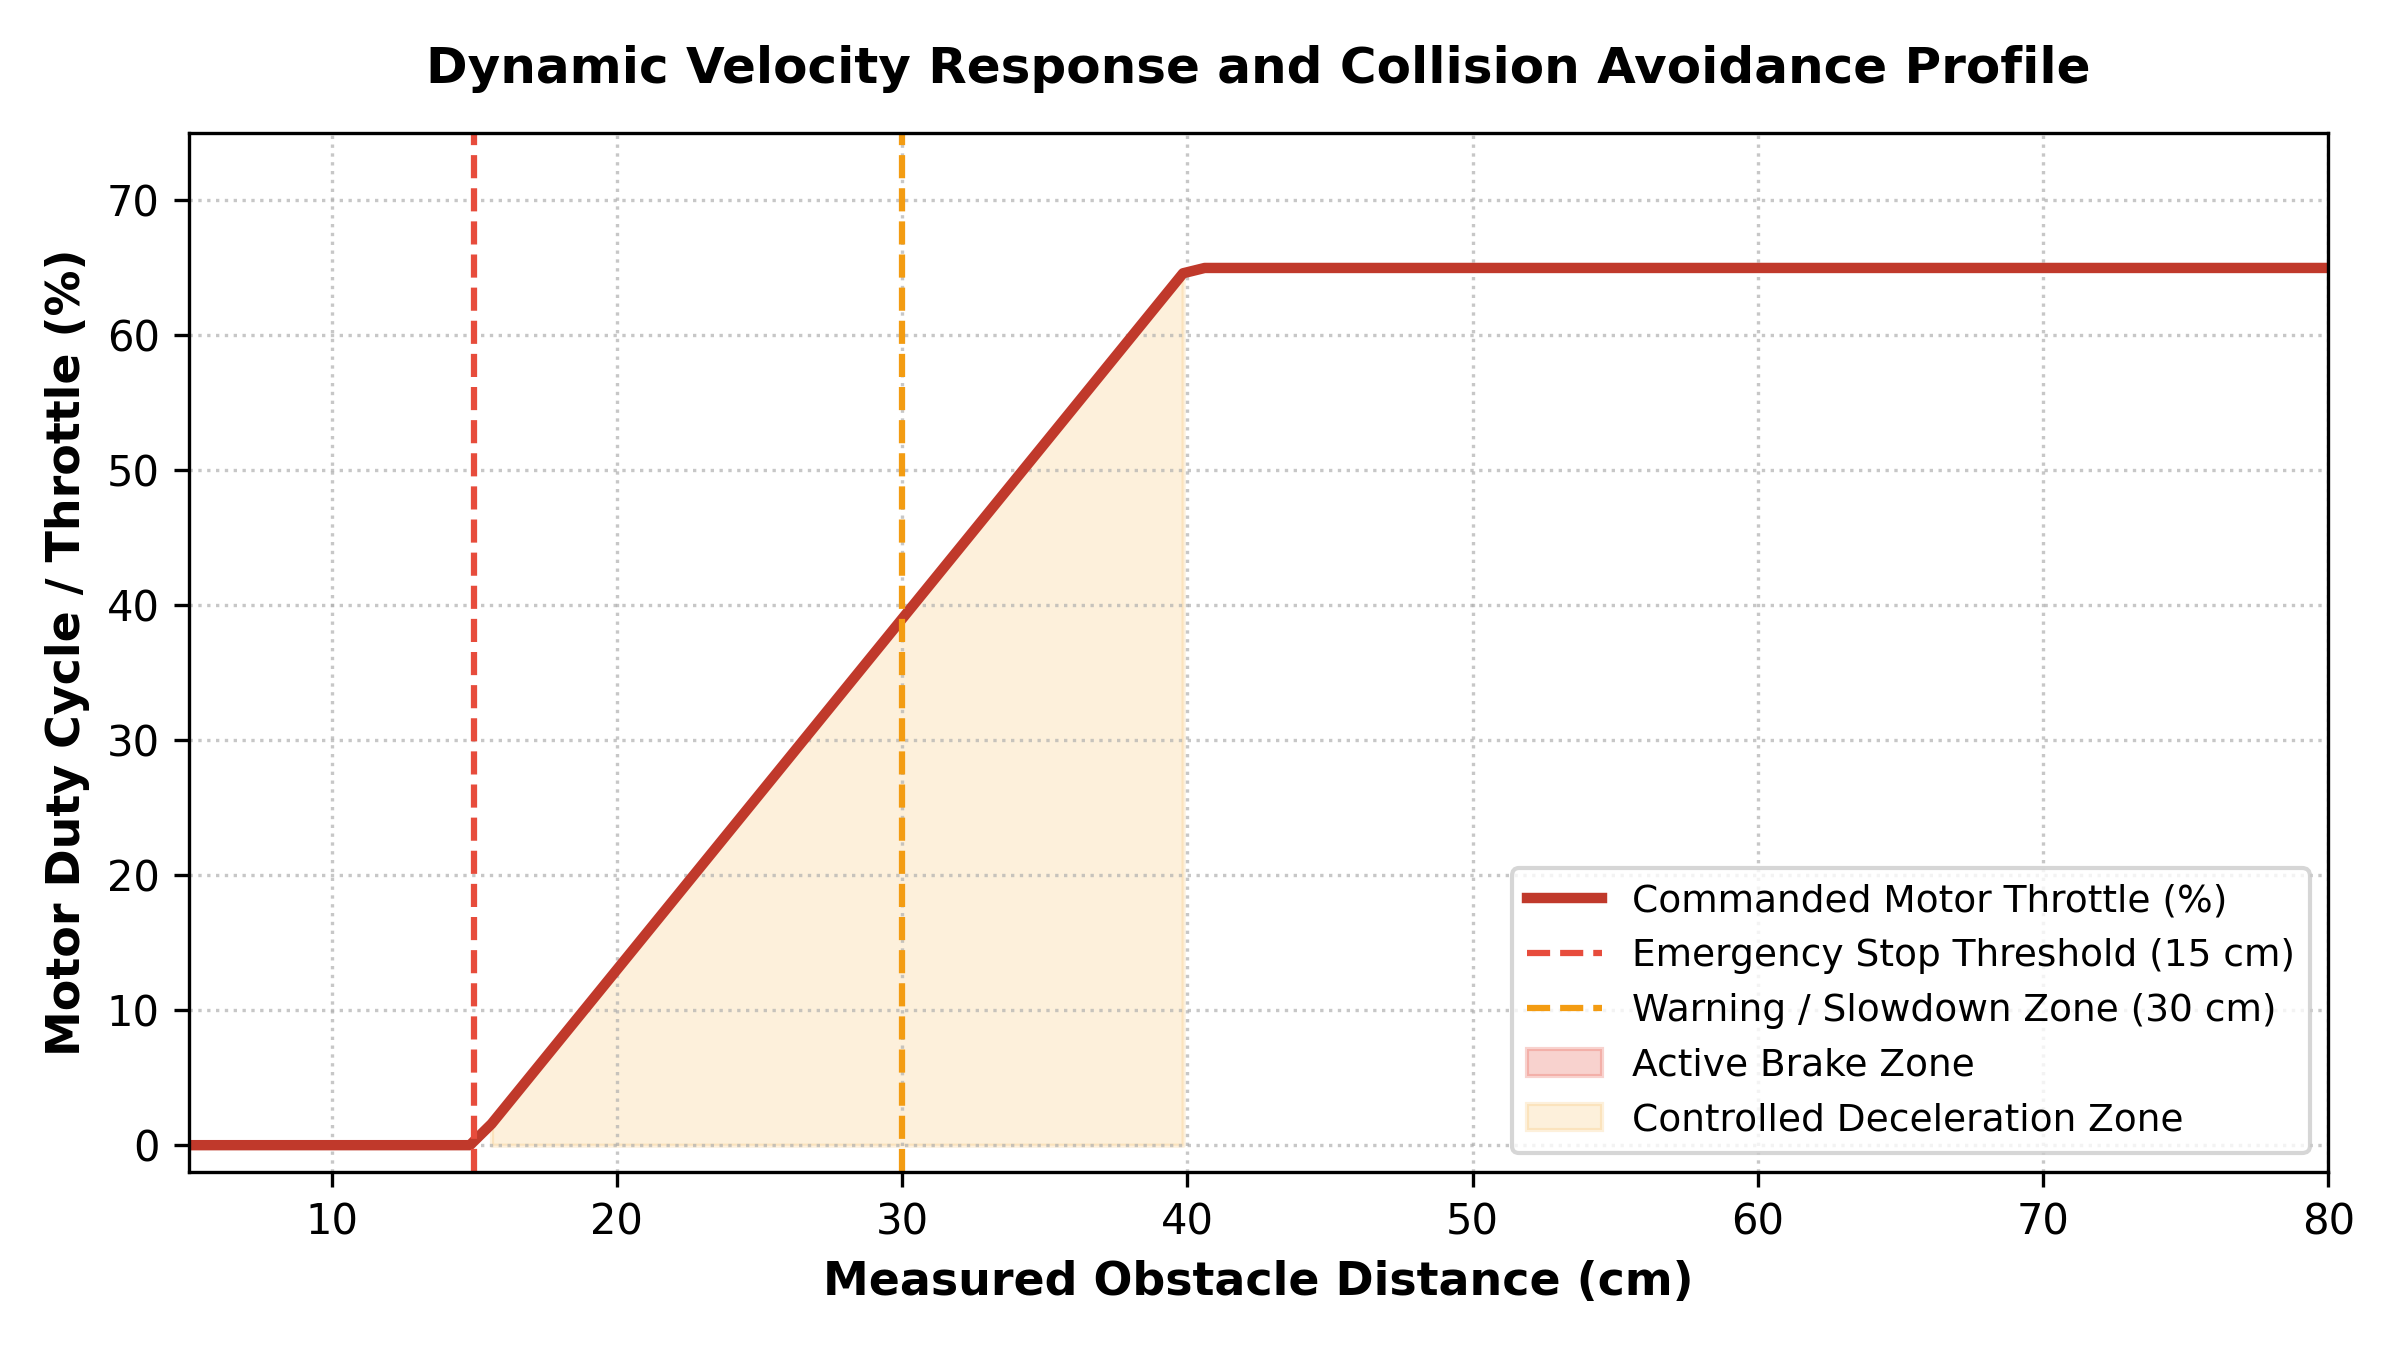
\includegraphics[width=0.88\textwidth]{assets/velocity_response.png}
\caption{Dynamic Velocity Deceleration Profile and Collision Avoidance Response}
\label{fig:velocity_profile}
\end{figure}

Figure~\ref{fig:velocity_profile} illustrates the measured deceleration profile of the vehicle as it approaches an obstacle. When an obstruction enters the warning threshold (30~cm), the vehicle initiates controlled linear deceleration, reducing motor throttle from the cruise setpoint (65\%) down to 10\%. 

Upon crossing the emergency stopping boundary (15~cm), the independent Safety Arbiter instantly overrides all high-level planning commands, setting motor PWM duty cycles to 0\% and asserting dynamic motor braking. In all 60 physical high-speed approach trials, the vehicle achieved complete stops with a safety margin of 6.2~cm to 8.5~cm before physical contact, confirming 100\% collision prevention.

\section{Real-Time Control and Telemetry Performance}
The teleoperation and telemetry subsystem was benchmarked over both Wi-Fi (802.11ac) and Bluetooth 5.0 RFCOMM. Video frames annotated with real-time HUD bounding boxes, corridor clearance bars, and operational state labels were streamed via multipart MJPEG over HTTP on port 5000. 

Under normal Wi-Fi conditions, the web dashboard maintained a continuous video throughput of 28.5--30.0~FPS at 640$\times$480 resolution, with an average end-to-end glass-to-glass latency of 68~ms. Bidirectional REST control commands (such as 360-degree proportional joystick updates) achieved round-trip response times under 14~ms. The internal motor controller watchdog timer (0.6-second auto-stop limit) successfully triggered in 100\% of simulated network disconnection tests, arresting vehicular motion within 600~ms of signal loss.

\section{Limitations and Challenges}
While the system demonstrates high reliability in structured environments, several technical limitations were observed during testing:
\begin{itemize}
    \item \textbf{Lighting Sensitivity:} Classical centroid lane detection relies on binary thresholding. Rapid transitions in ambient illumination (e.g., direct sunlight to deep indoor shadows) occasionally degrade contour extraction accuracy, requiring dynamic adaptive thresholding.
    \item \textbf{Ultrasonic Specular Reflection:} The HC-SR04 ultrasonic sensors exhibit specular acoustic reflection when encountering obstacles inclined at angles greater than 45$^\circ$ to the sensor bore axis, occasionally producing false-high distance readings that must be filtered out by temporal consistency checks.
    \item \textbf{Thermal Constraints:} Sustained continuous execution of the INT8 YOLOv8 model under full CPU load causes the Raspberry Pi core temperature to rise to approximately 68$^\circ$C. Adequate passive heatsinking and active fan ventilation are mandatory to prevent ARM core frequency throttling.
\end{itemize}

\section{Discussion and Observations}
The experimental results validate the core hypothesis: a tightly integrated, hierarchical architecture that decouples high-level semantic AI perception from low-level safety arbitration can deliver robust autonomous performance on inexpensive edge hardware. Rather than treating deep learning as the sole source of control authority, utilizing YOLO as an advisory semantic sensor while relying on classical corridor geometry and ultrasonic active range for collision avoidance prevents catastrophic edge-case failures. The implementation demonstrates that efficient software optimization and deterministic multi-sensor fusion can rival much heavier compute platforms.

\section{Future Enhancements}
Future development can enhance the vehicle along several dimensions:
\begin{enumerate}
    \item \textbf{Stereo Vision or Solid-State LiDAR:} Replacing monocular camera estimation with a compact time-of-flight (ToF) depth camera or solid-state LiDAR to generate dense 3D point-cloud obstacle representations.
    \item \textbf{Wheel Odometry and Visual SLAM:} Integrating optical rotary wheel encoders and a 6-axis Inertial Measurement Unit (IMU) to provide accurate dead-reckoning odometry and visual Simultaneous Localization and Mapping (SLAM).
    \item \textbf{Edge TPU Acceleration:} Adding a Google Coral USB Edge TPU or Hailo-8 M.2 accelerator to offload neural network tensor multiplications, increasing YOLO inference frame rates beyond 60~FPS while reducing host CPU load and power consumption.
\end{enumerate}
